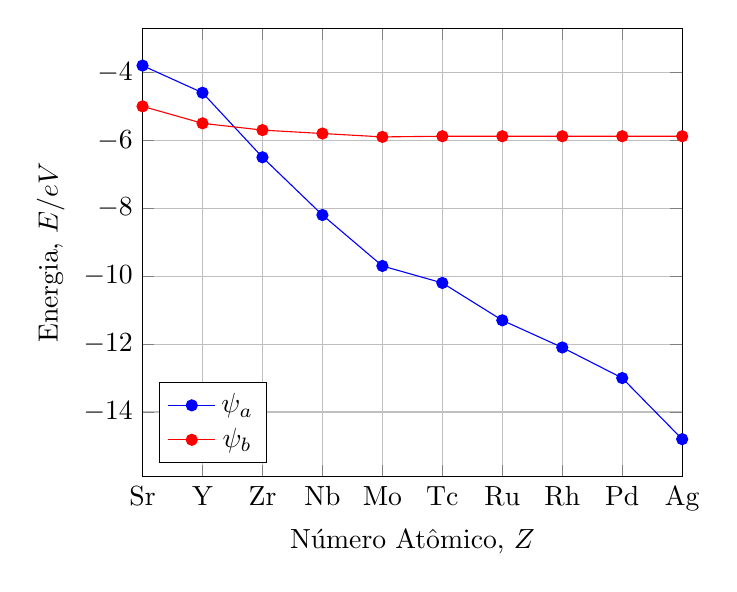
\begin{tikzpicture}
    \begin{axis}
        [
            grid=major,
            legend pos = south west,
            xlabel = {Número Atômico, $Z$},
            ylabel = {Energia, $E/\si{eV}$},
            xmin={0}, xmax={9},
            xtick={0,1,2,3,4,5,6,7,8,9},
            xticklabels={\ce{Sr}, \ce{Y}, \ce{Zr}, \ce{Nb}, \ce{Mo}, \ce{Tc}, \ce{Ru}, \ce{Rh}, \ce{Pd}, \ce{Ag}}
        ]
    \addplot[mark=*,color=blue] coordinates
        {
            (0,-3.8)
            (1,-4.6)
            (2,-6.5)
            (3,-8.2)
            (4,-9.7)
            (5,-10.2)
            (6,-11.3)
            (7,-12.1)
            (8,-13)
            (9,-14.8)
        };
    \addplot[mark=*,color=red] coordinates
        {
            (0,-5)
            (1,-5.5)
            (2,-5.7)
            (3,-5.8)
            (4,-5.9)
            (5,-5.88)
            (6,-5.88)
            (7,-5.88)
            (8,-5.88)
            (9,-5.88)
        };
    \legend{$\psi_a$,$\psi_b$}
    \end{axis}
\end{tikzpicture}